\documentclass[12pt, letterpaper]{amsart}%{scrartcl}
\usepackage[utf8]{inputenc}
\usepackage{graphicx}
\usepackage{amsmath} % Math package. E.g. piecewise functions.
\usepackage[hidelinks]{hyperref} %For hyperlinks, [hidelinks] is to take away link boarders.
\usepackage{threeparttable} % To make notes under tables.

\usepackage{csquotes} % Used for displaying the quote using \begin{displayquote}

\usepackage{float}
\restylefloat{table}

\usepackage{csvsimple} % Package for making csv tables

\interfootnotelinepenalty=10000 % Prevent footnote from breaking to another page

\usepackage{setspace,kantlipsum} % For line spacing.
%\usepackage[margin=2.5cm]{geometry} % Changing the margins.


\begin{document}

\begin{titlepage}
\begin{center}

\centering 

\includegraphics[scale=0.2]{LundUniversity_C2line_BLACK.png}

\vspace{1cm}

\Large{On stock return prediction with LSTM networks}

\vspace{0.5cm}

\large{Magnus Hansson}

\small{hansson.carl.magnus@gmail.com}

\vspace{1cm}

supervised by\par 
Prof. Birger Nilsson

\vspace{1cm}

\small{Department of Economics}
\\
\small{Lund University}

\vspace{1cm}

\large{Seminar: $1^{st}$ of June 2017, 4:15 pm, EC1:270 Lund}
\end{center}

\vspace{1cm}

\small{\textbf{Abstract.} Artificial neural networks are, again, on the rise. The decreasing costs of computing power and the availability of big data together with advancements of neural network theory have made this possible. In this thesis, LSTM (long short-term memory) recurrent neural networks are used in order to perform financial time series forecasting on return data of three stock indices. The indices are S\&P 500 in the US, Bovespa 50 in Brazil and OMX 30 in Sweden. The results show that the outputs of the LSTM networks are very similar to those of a conventional time series model, namely an ARMA(1,1)-GJRGARCH(1,1), when a regression approach is taken. However, they outperform the time series model with regards to direction of change classification. The thesis shows significant results for direction of change classification for the small Swedish market, and insignificant results for the large US market and the emerging Brazilian market. When a trading strategy is implemented based on the direction of change, a deep LSTM network vastly outperforms the time series model.}

\vfill

\small{\textbf{Key words:} artificial neural networks, recurrent networks, LSTM, EMH}
\end{titlepage}

\newpage


\newpage
\tableofcontents
\newpage
%\begin{spacing}{1.5}

\section*{Glossary}
\noindent
\textbf{Artificial neural network} $\cdots$ A numerical approximation method.
\\

\noindent
\textbf{Activation function} $\cdots$ A function that is wrapped around a node (neuron) in a neural network. The choice of this function(s) dictates in large parts what properties a network will exhibit.
\\

\noindent
\textbf{Backpropagation} $\cdots$ An algorithm which calculates the derivatives of the error function of the network.
\\

\noindent
\textbf{Batch} $\cdots$ The training data is divided into batches. Theoretically one can feed all the training data into a network at once, but practically it is limited to the computer's memory.
\\

\noindent
\textbf{Deep network} $\cdots$ Artificial neural network with multiple hidden layers, i.e. more adjustable parameters/higher degrees of freedom.
\\

\noindent
\textbf{Deep learning} $\cdots$ Machine learning with deep networks.
\\

\noindent
\textbf{Epoch} $\cdots$ Passing the input data through the network and optimizing the weights once, is one \textit{epoch}.
\\

\noindent
\textbf{Error function} $\cdots$ $E(\bold{y},\bold{t})$, where $\bold{y}$ is the output of the network and $\bold{t}$ is some target value. Minimizing the error function is equal to training the network. An example of an error function is \textit{mean squared error}, $MSE = \frac{1}{n} \sum_{i=1}^n (y_i - t_i)^2$.
\\

\noindent
\textbf{Feedforward network} $\cdots$ A simple network structure. Input data is fed into the network in one end, processed by the network and comes out as output in the other end.
\\

\noindent
\textbf{Hidden layers} $\cdots$ The network layers between the input layer and the output layer. They are called \textit{hidden} layers because they are not directly observed, unlike the input and output layer.
\\

\noindent
\textbf{Learning rate} $\cdots$ The rate at which an optimization algorithm travels forward in order to find a minimum or maximum.
\\

\noindent
\textbf{LSTM network} $\cdots$ A recurrent network structure which identifies autoregressive properties in the data of arbitrary length.
\\

\noindent
\textbf{Machine learning} $\cdots$ Methods in which an algorithm \textit{learns}, i.e. optimizes parameters, in order to perform a task. 
\\

\noindent
\textbf{Network training} $\cdots$ Optimizing the adjustable parameters of a neural network. 
\\

\noindent
\textbf{Non-convex optimization} $\cdots$ Optimizing functions which are non-convex. When numerically optimizing non-convex functions there is no guarantee that one arrives at the global minimum/maximum. Thus, programming algorithms for these type of problems require some thought.
\\

\noindent
\textbf{Recurrent neural network} $\cdots$ This network structure is different from a feedforward structure. Data is reprocessed by the hidden layers within the network.
\\

\noindent
\textbf{Regularization} $\cdots$ A term used in machine learning to describe the process of preventing over-fitting of the training data.
\\

\noindent
\textbf{Weights (w) \& biases (b)} $\cdots$ These are the adjustable parameters of a neural network. One can think of them as $k$ and $m$ in $y = kx+m$.

\newpage

\section*{Abbreviations}
\noindent
\textbf{AI} $\cdots$ Artificial intelligence.
\\

\noindent
\textbf{ANN} or \textbf{NN} $\cdots$ Artificial neural network.
\\

\noindent
\textbf{API} $\cdots$ Application programming interface.
\\

\noindent
\textbf{ARMA} $\cdots$ Autoregressive moving average.
\\

\noindent
\textbf{EHM} $\cdots$ Efficient market hypothesis.
\\

\noindent
\textbf{GARCH} $\cdots$ Generalized autoregressive conditional heteroskedasticity.
\\

\noindent
\textbf{GJR-GARCH} $\cdots$ Glosten-Jagannathan-Runkle GARCH.
\\

\noindent
\textbf{LSTM} $\cdots$ Long short-term memory.

\newpage

\section{Introduction}
\begin{displayquote}
\textit{Artificial neural networks (NN) is a timely subject. This method emulates the brain's way of thinking. It has its input neurons, which feed the neural network with descriptors values, the hidden layers that weight and mix the incoming signals, and an output layer with neurons predicting the calibrated response values.}
\end{displayquote}
\vspace{0.5cm}

This was written in my father's PhD thesis \textit{Quantitative Structure-Retention Relationships of Diastereomers in Reveres-Phase Liquid Chromatography} in $1993$. Although the information in the quote still holds true, and the core structure of a neural network is as described, extensive advances have been seen in the subject since then. New areas of application have also arisen. With higher computing power and high level APIs, deep learning\footnote{Deep learning refers to the training of neural network with multiple hidden layers.} is now possible in a way it has never been before.
\\

In this thesis forecasting of financial returns series will be investigated through a comparison of LSTM (long short-term memory) recurrent neural network models and conventional state of the art financial econometric models. Accurately forecasting financial time series is notoriously hard, due to its obvious reasons. However, evaluating the weak form of the efficient market hypothesis with a new and highly nonlinear method, such as LSTM's, is interesting.
\\

From here on the terms artificial neural network, neural network, neural net, ANN, NN, network etcetera will be used interchangeably.

\subsection{Artificial neural networks}
Artificial neural networks had its name from mathematicians trying to build a model mimicking the neural activity in a brain. In 1943 a quite famous article named \textit{A Logical Calculus of the Ideas Immanent in Nervous Activity} was written. The article discussed the first properties that were later to be coined as an \textit{artificial neural network}. In 1962, Rosenblatt presented single layer neural networks with threshold activation functions\footnote{An activation function is wrapped around each node (neuron) in the network, $g(\cdot)$ in equation (3) is an example of this.}. These are essentially feedforward neural networks which will be explained later (section 3.2 and 3.3), however they use a specific activation function. During this time neural networks where interesting from a biological and mathematical perspective, but had little practical use since computing power was expensive and unavailable. This led to advancements in the mathematical theory of neural nets. One of the interesting discoveries was the \textit{universal approximation theorem} proven by (e.g.) Cybenko (1989). Cybenko proved that a single hidden layer neural network, given the sigmoid activation function, could approximate any continuous function arbitrary well. This result was quite restrictive since the sigmoid function was assumed. Hornik (1991) was able to prove the theorem for an arbitrary bounded activation function.
\\


During the last twenty years neural networks have had an enormous advancement in a variety of fields. The most distinguishable areas have been within traditional machine learning (such as classification and data analysis) and artificial intelligence during the last ten years. A large number of APIs for neural network applications have been developed for numerous computer languages, one example is Google's \textit{Tensorflow}. This in combination with the rapid development of computing power have led to the use of neural networks in our everyday life. One can see the use of neural nets when using Google translate, a huge number of mobile phone applications (e.g. apps with facial recognition), or self driving cars.

\subsection{Neural networks within finance}
Neural nets have been applied within finance for a long time. Twenty years ago networks with feedforward structure and often only one hidden layer were used (Fadlalla \& Lin 2001). These networks outperformed the simple linear regressions and some traditional statistical methods because of the nonlinear nature of financial data and the networks abilities to \textit{see through} distorted data. Applications were, e.g., found within forecasting of T-bills, asset management, portfolio selection and fraud detection. Since neural nets have the ability to heavily generalize the structure of the input data it has been shown to be robust when measuring bankruptcy risk. Other areas of application are e.g. bond rating, risk management, financial forecasting and stock market prediction (Johnson \& Whinston 1994).
\\

Several deep learning studies have been made during the last years with applications within finance and financial econometrics. The major reason for this is the same as the reason why neural networks are frequently used within other fields at the moment - data has grown larger and computing power has become more accessible. Neural network models have also been seen in trading lately. Although quantitative trading firms keep their algorithms secret there are websites such as Kaggle \footnote{\url{https://www.kaggle.com/}} and Quantopian \footnote{\url{https://www.quantopian.com/}} where quantitative trading is discussed and practiced.

\subsection{Purpose}
The rise of sophisticated sequential\footnote{Sequential modeling takes time into consideration.} neural network models give reason to again investigate the Efficient Market Hypothesis (EHM). Can these models, with their high degree of nonlinearity, utilize historical data in order to predict market returns? Furthermore, do the methods perform differently on different (e.g. large, emerging and small) markets?
\\

The purpose of this thesis is to investigate the weak form of the Efficient Market Hypothesis (EMH) on the American, Brazilian and Swedish stock markets using both conventional time series modeling and highly nonlinear recurrent neural network modeling.
\\

Questions that will be answered:
\\

\begin{itemize}
\item Can the American, Brazilian or Swedish stock market returns be predicted using LSTM's?
\item Can the directions of the market returns be predicted using LSTM's?
\item Can LSTM neural nets compete with conventional time series models?
\item Is predictability of market returns different for America, Brazil and Sweden?
\item Is it possible to build a successful financial trading strategy based on LSTM network prediction?
\end{itemize}
\vspace{0.5cm}

\subsection{Some related research}
Gencay (1996) and Gencay \& Stengos (1998) examine how simple feedforward networks performs compared to an ARMA(1,1)-GARCH(1,1) model. They use moving-average indicators as inputs into the networks. Furthermore, they claim that the networks perform better than the ARMA(1,1)-GARCH(1,1) model when adopting buy/sell strategies. Both articles use daily Dow Jones Industrial Average Index data between 1963 and 1988.\footnote{Using data that is \textit{old}, i.e. before the evolution of big data and modern technology, might alter the relevance of a significant result.}
\\

Enke (2005) uses a feedforward neural network model together with a data mining\footnote{Methods of discovering patterns in large datasets.} framework in order to investigate predicting power of the input variables. He shows that given the right inputs a neural network model outperforms a buy and hold strategy. Qiu, Song and Akagi (2016) investigates the same problem but also how the result differs with different optimization methods. However most research uses neural nets of feedforward architecture Maknickiene et al. (2011) is one example where they use recurrent networks for financial analysis. Rutkauskas (2010) is another example where LSTM networks are used to find a model for asset return prediction.
\\

Because accurately predicting stock market returns is challenging a more simple binary classification method is often used. This is called \textit{direction of change forecasting}, and tries to predict the direction of the market rather than the direction and magnitude. An interesting paper is Christoffersen et al. (2006) where they investigate the link between sign forecasting and the conditional variance, mean, skewness and kurtosis\footnote{Christoffersen et al. (2006) investigates direction of change forecasting based on conditional variance, mean, skewness and kurtosis. They verify that higher order moments are an important factor for sign forecasting. This is an interesting result since neural networks take all factors concerning the empirical distribution into account. The more unusual relationships not described by regular models the better is the relative performance of a NN.}. More often are papers investigating the volatility of market returns which is easier to predict. For example see Mantri, Gahan \& Nayak 2010 and Hu \& Tsoukalas 1999.

\subsubsection{Thesis positioning}
There are little research done on forecasting of stock market returns and its direction of change using long short-term memory (LSTM) recurrent neural networks. Although, LSTM's have been around since 1997 they have recently become popular because of the new AI wave, and the availability of programming interfaces that can handle them. In this thesis two different LSTM models, with two different activation functions, yielding four different models are used on three different datasets which exhibits different market characteristics. Thus, the experiment will yield interdisciplinary results regarding classic financial empirics, such as application of the efficient market hypothesis (section 2.2) and advanced modern machine learning.

\subsection{Thesis outline}
Section 2 covers some financial theory needed for the empirical analysis. Section 3 discusses the mathematical concepts which are in the core of the neural network models and some time series econometrics. Section 4 describes the empirical experiment and show its results. In section 5 the results are discussed and in section 6 some final conclusions are drawn.

\section{Financial theory}
When performing a quantitative analysis which includes empirics, the understanding of the data is of high importance. In this part some financial theory is presented in order to clarify the empirical methodology later. Section 2.1 is discussing stylized facts about univariate return series and 2.2 is discussing the EMH (efficient market hypothesis).

\subsection{Stylized facts of univariate return series}
When looking at the study of empirical finance and more specifically empirical finance using financial returns, it is clear that there are some general statistical properties of these time series. Campbell et al. (1997) is one example discussing several properties, and referring to Rama Cont (2000) one can summarize a set of stylized facts regarding univariate return series.
\\

\begin{itemize}  
\item No linear autocorrelation.
\item Slow decay of linear autocorrelation of absolute returns.
\item Heavy tails.
\item Larger tail for losses than for positive returns.
\item The shape of the distribution changes through time.
\item Volatility clustering.
\item Conditional heavy-tails (even after adjusting for volatility clustering).
\item Leverage effect. Volatility is negatively correlated with returns.
\item Correlation between trading volume and volatility.
\end{itemize}
\vspace{0.5cm}

When modeling financial returns one has to take into account the distributional characteristics of the data. Fitting financial return data under a normal i.i.d.\footnote{Independent and identically distributed.} assumption is usually not best practice. Taking into account the autoregressive properties of the underlying error variance is usually good practice. Hence, this is highly important when choosing time series models representing the data. However, when modeling data using neural nets one does not need to take any distributional assumptions into account, given that the practitioner knowns how to analyze the output. This is due to the general way in which a neural net learns the empirical distribution of the training data.

\subsection{Efficient market hypothesis}
The EMH argues that markets are efficient, which means that all available information is reflected in the prices of assets. The issues of predicting prices and the EMH has been widely researched. Martin Sewell refers back to the mathematicians of Italy in the $16^{th}$ century (Martin Sewell 2011). If one does not look back quite as long, but rather to the 1970's, a classical paper written by Eugene Fama is found. He defines a market with respect to some information set to be efficient if the prices fully reflects that information set (Fama 1970).
\\

Looking at Roberts (1967), we see three different types of efficiencies: weak, semistrong and strong. These are defined with respect to the information set, where the weak form refers to an information set which consists of historical data. The semistrong form of efficiency refers to the information set including all public information. In the definition of the strong form of market efficiency the information set consists of all information known to any market participant. Thus, this thesis is concerned with the \textit{weak} form of the EMH.

\section{Mathematical background}
The mathematical background is introduced with the \textit{universal approximation theorem} in section 3.1. The theorem is followed by a description of single- and multi-layer feedforward neural networks, in sections 3.2 and 3.3. Neural network training is discussed in 3.4. A short section on regularization is presented in 3.5, followed by recurrent neural networks in 3.6. The last section, 3.7, is concerned with some time series econometrics. The notation in the mathematical background is based on Bishop (1995) and Enders (2015).

\subsection{Universal approximation theorem}
There are several versions of the universal approximation theorem. All saying that a single hidden layer feedforward network with an arbitrary number of hidden nodes can approximate any given continuous function under some assumptions. However, each version have slightly different assumptions. One of the first versions of the theorem was proven by Cybenko (1989). Cybenko proved the theorem for the sigmoid function as activation function. Later, Hornik (1991) showed that the theorem holds for an arbitrary function given some assumptions. One of Horniks assumptions was that the activation function needed to be bounded, which e.g. prohibits the ReLU (rectified linear unit function) to be used. \footnote{The ReLU function, defined as $f(x) = max(0,x)$ has become an important activation function within deep networks. The reason for this is its derivative which is either $0$ or $1$. Other popular activation functions, such as the sigmoid function $s(x) = \frac{1}{1 + e^{-x}}$, has derivative close to zero for small and large values of $x$. Because the optimization consists of multiplication of several derivatives due to \textit{backpropagation} (section 3.4) a problem known as \textit{vanishing gradient} present itself when multiplying many small derivative together. However this problem is non-existing using the ReLU function, thereof its popularity.} Sonoda \& Murata (2015) investigated the theorem for an unbounded function, since the ReLU function is state of art within deep learning, and indeed showed that the theorem still holds for unbounded functions.
\\

One compact version of the theorem is found in Haykin (1998) and builds upon Hornik's foundings,

\newtheorem*{mydef}{Universal approximation theorem}

\begin{mydef}
Let $\varphi (\cdot)$ be a bounded, and monotone-increasing continuous function. Let $I_{D}$ denote the $D$-dimensional unit hypercube $[0,1]^{D}$. The space of continuous functions on $I_{D}$ is denoted by $C(I_{D})$. Then, given any function $f \in C(I_{D})$ and $\epsilon > 0$, there exist an integer $M$ and sets of real constants, $\alpha_j, b_j, w_{ij}$, where $j = 1, ...,M$ and $i = 1, ...,D$ such that we may define

\begin{equation}
    F(x_1, ..., x_{D}) = \sum_{j=1}^{M} \alpha_j \varphi \left( \sum_{i=1}^{D} w_{ij} x_i + b_j \right)
\end{equation}

as an approximate realization of the function $f(\cdot)$; that is,

\begin{equation}
    \vert F(x_1, ..., x_{D}) - f(x_1, ..., x_{D}) \vert < \epsilon
\end{equation}

for all $x_1, x_2, ..., x_{D}$ that lie in the input space.

\end{mydef}

\subsection{Single-layer feedforward networks}
Consider the following equation describing a single layer network,

\begin{equation}
y_k = g \left( \sum_{i=0}^D w_i x_i \right)
\end{equation}

where $y_k$ is the output, $g(\cdot)$ is an activation function, $x_i$ is input and $w_i$ is its corresponding weights. $x_0 = 1$ which consequently makes $w_0$ a bias parameter. This means that by setting $x_0=1$ a bias parameter is added, one can compare this to the $b$ in $y = ax + b$. These biases are, like the rest of the weights, adjustable parameters within the network.
\\

With some imagination one could think of the activation function, $g(\cdot)$, as giving equation $(3)$ different characteristics. If $g(\cdot)$ takes the from of a simple linear function\footnote{I.e. the identity function, $g(a)=a$.}, equation $(3)$ simply becomes a linear regression. If $g$ is the binary function given by,

\begin{equation}
g(a) = 
     \begin{cases}
       1 \ \text{if} \ a > 0 \\
       0 \ \text{otherwise} \\ 
     \end{cases}
\end{equation}

equation $(3)$ becomes a classifier of the type \textit{Perceptron}. If $g(\cdot)$ instead takes the form of the non-linear \textit{logistic sigmoid} function\footnote{$s(a) = \frac{1}{1+e^{-a}}$.} it becomes a logistic regression.
\\

Depending on how the activation function, which wraps the linear expression, is defined, the network is given different characteristics. This gives an intuition behind the generality of neural networks.

\subsubsection{Drawbacks of a single-layer network}
Considering a classification problem of two classes, a single-layer neural network can only classify data sets which are linearly separable. This means that one, in $two$-dimensions, can draw a line between the classes. This problem is usually illustrated with the \textit{XOR} example\footnote{Imagine a two-dimensional plane where the points $x_1 = (0,1)$ and $x_2 = (1,0)$ are categorized by class 1, $\mathbf{C_1}$. Likewise, the points $y_1=(0,0)$ and $y_2=(1,1)$ are categorized by class 2, $\mathbf{C_2}$. Then there is no line separating the two classes.}. The limitation of a single-layer network can also be exemplified given a regression example, in which the dimensionality of the linear expression inside the activation function is a restriction. In general, single-layer neural networks are not used in practice, but used to illustrate the concept of NN. 


\subsection{Multi-layer feedforward networks}
Now, consider the following equation describing a multi-layer neural network with one hidden layer,

\begin{equation}
y_k = h \left( \sum_{j=0}^M w_{kj}^{(2)} g \left( a_j \right) \right)
\end{equation}

where,

\begin{equation}
a_j = \sum_{i=0}^D w_{ij}^{(1)} x_i
\end{equation}

One can identify that the structure is the same as the single-layer network. One can also identify that equation (5) is in fact equal to equation (1) in the universal approximation theorem (section 3.1), given that $h$ is linear. Furthermore, the general difference from a single layer network is that the output of the inner layer is again multiplied by a new weight vector and again wrapped in an activation function. Notice that the output from the first layer is usually non-linear, meaning that the more layers the network consist of the more complex becomes the output.
\\

\textit{Figure 1} illustrates a network with two layers, where one is hidden. $x_i$ is the input data, $z_j = g(a_j)$ is the hidden nodes, and $y_k$ is the output. Hence, there are two layers of adaptive weights that will be optimized, these are represented by the lines.

\begin{figure}[h]%[H]
\caption{Network graph for one hidden layer network.}
\centering
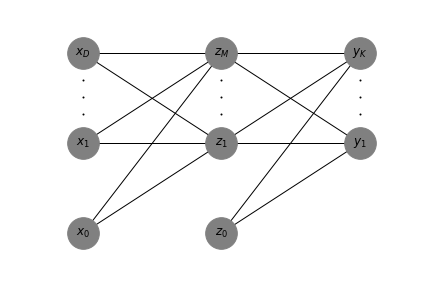
\includegraphics[scale=0.8]{Network.png}
\end{figure}

%\begin{center}{Figure 1. Network graph for one hidden layer network.}
%  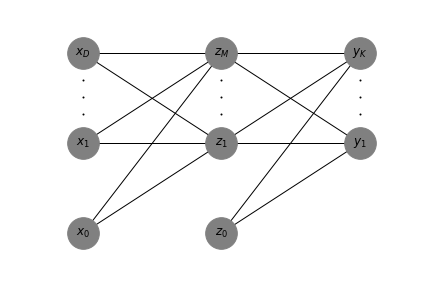
\includegraphics[scale=0.8]{Network.png}
%\end{center}

\subsection{Network training}
The network training can be described by defining an error function, and utilizing backpropagation with gradient descent. Backpropagation is the method of backwards, through the network, finding the gradient of the error function. Gradient descent is simply the numerical method for optimizing the weights.

\subsubsection{General derivation of backpropagation}
Consider the following sum,

\begin{equation}
    a_j = \sum_i w_{ji}z_i
\end{equation}

This sum is a representation of a network layer, where $w_{ji}$ is the weights and $z_i$ is the input. If $z_i$ happens to be the network input it is called $x_i$, and if it is the network output it is called $y_i$. Now consider,

\begin{equation}
    z_j = g(a_j)
\end{equation}

where the layer is again wrapped by an activation function. In order to optimize the weights one must define a suitable error function\footnote{An usual error function when training regressional neural networks is \textit{mean squared error}, $MSE = \frac{1}{n} \sum_{i=1}^n (\hat{y}_i - y_i)^2$.} and find its derivatives.

\begin{equation}
    E = \sum_i E^n
\end{equation}

Furthermore, 

\begin{equation}
    E^n = E^n(y_1,...,y_c)
\end{equation}

Now, lets look at the derivative of the error with respect to some weight. Using the chain rule,

\begin{equation}
    \frac{\partial E^n}{\partial w_{ji}} = \frac{\partial E^n}{\partial a_j} \frac{\partial a_j}{\partial w_{ji}}
\end{equation}

The first part of the right hand side is known as the \textit{delta}'s ,

\begin{equation}
    \delta_j \equiv \frac{\partial E^n}{\partial a_j}
\end{equation}

The second part of the right hand side of equation (11) clearly becomes,

\begin{equation}
    \frac{\partial a_j}{\partial w_{ji}} = z_i
\end{equation}

by utilizing equation (7). Lets rewrite (11),

\begin{equation}
    \frac{\partial E^n}{\partial w_{ji}} = \delta_j z_i
\end{equation}

This means that to evaluate the derivatives of the error function one only has to multiply the \textit{delta}'s with the inputs. The delta's for the output layer become,

\begin{equation}
    \delta_k \equiv \frac{\partial E^n}{\partial a_k} = g \prime (a_k) \frac{\partial E^n}{\partial y_k}
\end{equation}

The delta's for the hidden layers are,

\begin{equation}
    \delta_j \equiv \frac{\partial E^n}{\partial a_j} = \sum_k \frac{\partial E^n}{\partial a_k} \frac{\partial a_k}{\partial a_j}
\end{equation}

Now consider the general algorithm for backpropagation,

\begin{equation}
    \delta_j = g \prime (a_j) \sum_k w_{kj} \delta_k
\end{equation}

The backpropagation formula propagates back through the network in order to evaluate the gradient. The variation in $a_j$ goes through $a_k$. At a first glance this may seem complicated but the delta's for the output layer are known, and one can therefore recursively use the backpropagation formula (17) to evaluate the gradient for any network of feedforward structure. Once one batch of the dataset has been fed into the network and backpropagation has been preformed together with an optimization algorithm, one \textit{epoch} is completed. The idea of recursively using the chain rule to solve numerical optimization problems was first introduced in 1970 by Seppo Linnainmaa (Andreas Griewank 2010).

\subsubsection{Gradient descent}
The backpropagation algorithm finds the gradient of the error function, however an algorithm for optimization is needed. Analytically one would like to find for which set of weights, $\bold{w}$, $\nabla E=0$. It is not possible to find, $\bold{w}$, due to the dimensionality of the problem. Thus, the gradient descent algorithm is used to come as close as possible. The method starts with a random weight vector, $\bold{w}^{(0)}$, and evaluates the gradient of the error function at that point. Then the algorithm takes a small step, $\tau$, in the opposite direction of the gradient, and again evaluates at the new point $\bold{w}^{\tau}$. This can be expressed as,

\begin{equation}
\triangle \bold{w}^{\tau} = - \eta \nabla E \vert_{\bold{w}^{\tau}}
\end{equation}

where $\eta$ is the learning rate. This simple algorithm has problems with non-convex optimization, which clearly the training of a neural network exhibits. However, there are some adjustments such as \textit{stochastic gradient descent} in order to over come this problem.

\subsection{Regularization}
Regularization in neural network terminology refers to the process of regulating network layers in order to prevent over-fitting. \textit{Dropout} is the most commonly used regularization method based on the simple idea that one shoots out (drops out) a percentage of neurons in each layer, randomly, in order to decrease the degrees of freedom (adjustable parameters) of the network. Imagine that you have $1 000$ observations in your training data, and the network consists of $1 000$ nodes. Then, the network can \textit{store} all input information and does not need to construct generalized ways to describe the data. If one takes away half of the nodes in each training step then the network will not be able to over-fit to the training data and will need to come up with intelligent ways to describe the data. This is of course beneficial when trying to forecast out of sample. The dropout method is usually only used when building deep nets, with a lot of adjustable parameters.

\subsection{Recurrent networks}
Recurrent neural networks is a class of neural networks which can be thought of by the concept of a feedback loop. When the data has been processed by one of the hidden layers in the network it is sent back and again processed by that layer together with the new input. There are several types of recurrent networks depending on how they are structured. One type of recurrent network is the LSTM (long short-term memory) network which will be discussed in section 3.6.1.
\\

Recurrent neural networks is used when the data is of sequential nature. Hence, for example time series data. If one believes that the data has some kind of autoregressive structure a recurrent neural network can be used. One example where recurrent networks are used is within natural language processing (NLP). Because languages are sequential, the two sentences \textit{Henry has a car} and \textit{Car has a Henry} is not equivalent, although containing the same words. Hence, the concept of time can be introduced into artificial neural networks.

\subsubsection{Long short-term memory}
As mentioned in the section about recurrent neural nets, the LSTM (long short-term memory) network is of recurrent type. The LSTM network was introduced in 1997 in the paper \textit{Long Short-Term Memory} by Hochreiter \& Schmidhuber. One of the advantages with the LSTM model compared to an usual recurrent network model is the ability to capture autoregressive structures of arbitrary length. The regular recurrent network needs a prior specification of how many '\textit{feedback loops}' that will be present, this is not required when dealing with LSTM networks.
\\

Instead of regular neural network nodes, a LSTM network consists of LSTM blocks. Consider the following system of equations,

\begin{equation}
\begin{cases}
f_t = g \left( W_f \cdot [x_t, h_{t-1}] + b_f \right)\\
i_t = g \left( W_i \cdot [x_t, h_{t-1}] + b_i \right)\\
o_t = g \left( W_0 \cdot [x_t, h_{t-1}] + b_0 \right)\\
c_t = f_t \circ c_{t-1} + i_t \circ tanh \left( W_c \cdot [x_t, h_{t-1}] + b_c \right)\\
h_t = o_t \circ tanh \left( c_t \right)
\end{cases}
\end{equation}

where $g(\cdot)$ is the sigmoid function\footnote{$g(x)=\frac{1}{1+e^{-x}}$}, $tanh(\cdot)$\footnote{$tanh(x)= \frac{e^x - e^{-x}}{e^x + e^{-x}}$} is the hyperbolic tangent, $x_t$ is the input vector, $h_t$ is the output vector, $c_t$ is a cell state vector. $W$ are weights as before and $b$ are biases. $f_t$, $i_t$ and $o_t$ are called gates of the block. Note that $\circ$ is not matrix multiplication but the Schur product, i.e. entry wise product.
\\

This system of equations (19) represent one LSTM block. One can see the recurrent properties of the block as $h_{t-1}$, i.e., the output vector for period $t-1$, is included in the calculation of the output vector $h_t$.
\\

The first gate of the LSTM block, $f_t$ is the \textit{forget gate}. This gate decided upon which information will be forgotten in the cell state, $c_t$. Notice how the linear expression is wrapped in a sigmoid function, which indeed is bounded between 0 and 1. If the optimization sets $f_t$ to 0 the value is \textit{forgotten} in the calculation. The input gate, $i_t$, regulates what new information will be stored in the cell state. $o_t$ is the output gate. The output vector $h_t$ is a combination of the output gate and the cell state which contains stored information.
\\

The key to understand LSTM network is to understand the activation functions. How these functions can help the blocks store and forget information. The optimization takes care of setting the adjustable parameters accordingly.

\subsection{Time series models}
In this part of the \textit{Mathematical background} some time series econometrics will be presented. Why? One may ask. The obvious answer is because a new methodology such as LSTM recurrent networks, needs to be compared with some already existing method. In the empirics part an ARMA-GJRGARCH model will be used. In subsection 3.7.1 the ARMA part of the model will be introduced and in 3.7.2 the GJRGARCH part will be introduced.

\subsubsection{ARMA}
If one combines an autoregressive model with $p$ lags, $AR(p)$, and an moving average model with $q$ lags, $MA(q)$, one obtains an $ARMA(p,q)$ model.

\begin{equation}
y_t = a_0 + \sum_{i=1}^p a_i y_{t-1} + \sum_{i=0}^q \beta_i \epsilon_{t-1} 
\end{equation}

Under the assumption that all characteristic roots are in the unit circle, equation (20) is an $ARMA(p,q)$ process (Enders 2015). Although, regarding financial returns one needs not to worry since they are generally stationary.

\subsubsection{GJRGARCH}
Recall the $8^{th}$ stylized fact in subsection 2.1, the \textit{leverage effect}. I.e. volatility is negatively correlated with returns. The regular GARCH model fail to incorporate this observation. Therefore the GJRGARCH model is often used when modeling financial returns. The model was introduced by Glosten et al. (1993) and can be expressed as,

\begin{equation}
\sigma_t^2 = \omega + (\alpha + \gamma I_{t-1}) \epsilon_{t-1}^2 + \beta \sigma^2_{t-1}
\end{equation}

where $I_{t-1}$ is an indicator function,

\begin{equation}
I_{t-1}(\epsilon_{t-1}) = 
     \begin{cases}
       \epsilon_{t-1} \ \text{for} \ \epsilon_{t-1} > 0 \\
       0 \ \text{otherwise} \\ 
     \end{cases}
\end{equation}


\section{Empirics}
In section 4.1 the methodology of the experiment is discussed, in 4.2 the datasets are presented. In sections 4.3 and 4.4 the neural network models and the time series models are presented. 4.5 and 4.6 handle results and evaluation of the predictions. In section 4.7 the results and evaluation of two trading strategies are presented.

\subsection{Methodology}
The empirical methodology is divided into four parts,
\\

\begin{itemize}  
\item Regression with LSTM network models. Predicting 1-day ahead market returns.
\item Classification with simple LSTM network models. Predict 1-day ahead direction of market returns.
\item Classification with sophisticated LSTM network models. Predict 1-day ahead direction of market returns.
\item Construction of two trading strategies.
\end{itemize}
\vspace{0.5cm}

As discussed, forecasting financial returns is nothing easy. Thus one might not expect grand results from a forecasting model with simple regression approach, as is in step 1. However, one idea would be to use the predictions of the forecasting models to classify only the direction of the market returns, \textit{direction of change forecasting}. In the second part of the methodology a simple model is established, which wraps a \textit{sign}-function \footnote{$g(R) = 
     \begin{cases}
       \ \ 1 \ \text{if} \ R > 0 \\
       -1 \ \text{otherwise} \\ 
     \end{cases}$} around the regressional outputs of models. In the third part more sophisticated neural network classification models will be used. Instead of a linear output the models will have a binary classification output, discussed in 4.3.1.
\\

In the fourth part of the experiment two trading strategies will be implemented. These strategies will be based on the classification predictions, rather than the regression. The first strategy will buy the stock indices when the models predict positive returns and not be in the market when the models predict negative returns. The second strategy will buy the indices when the models predict a positive outcome and short\footnote{Short selling means that one sells a position without owning the underlying asset. This can be done with the help of financial derivatives. E.g. if a stock index have a negative return of $1\%$, an agent with a short position in that index gains $1\%$.} the indices when the models predict a negative outcome. Hence, the first model will be less risky since the potential loss is theoretically only the invested amount, whereas the theoretical potential loss of the second strategy is unlimited. In section 4.7 the sophisticated classification LSTM network will be compared to the time series model based on these two strategies.
\\

In all parts of the experiment 33\% of the data will be saved for testing, and hence not used in the estimation process. The first part of the method will be evaluated using the sum of squared residuals, while the second and third part of the method will be evaluated using a binomial test. The trading strategies will simply be evaluated by out of sample return performance compared to a buy and hold position of the indices.

\subsection{Data}
In order to investigate the predictability of the American, Brazilian and Swedish stock exchanges the following indices are used in the empirical analysis,
\\

\begin{itemize}
\item S\&P 500 index
\item Bovespa 50 index
\item OMX 30 index
\end{itemize}
\vspace{0.5cm}

where daily adjusted closing prices are imported and transformed into logarithmic returns. Due to reproducibility, simplicity and overall promotion of open data, the adjusted closing price are imported from Yahoo!'s finance database. \textit{Figure 2} shows a visualization of the return series of the indices together with histograms for each series. Table 1 and 2 shows a summary of the logarithmic returns, which will be analyzed.
\\

\begin{table}[h]%[H]
\centering
\caption{Summary of logarithmic returns (S\&P 500, Bovespa, OMX).}
\csvautotabular[separator=semicolon]{summary.csv}
\end{table}

Normally distributed data is symmetric around the mean, hence the skewness parameter is 0. The skewness parameters for the S\&P 500 index and the OMX index are negative, this means longer negative tails. The skewness parameter for the Bovespa index is positive implying longer positive tail. The kurtosis of each series exceeds 3, indicating excess kurtosis compared to the normal distribution. This is in accordance with the $3^{rd}$ stylized fact in section 2.1, i.e. \textit{heavy tails}.

\begin{table}[h]%[H]
\centering
\caption{Standard deviation and standardized moments of logarithmic returns (S\&P 500, Bovespa, OMX).}
\csvautotabular[separator=semicolon]{summary2.csv}
\end{table}

\begin{figure}[h]%[H]
\caption{Histograms \& plots of return series (S\&P 500, Bovespa, OMX).}
\centering
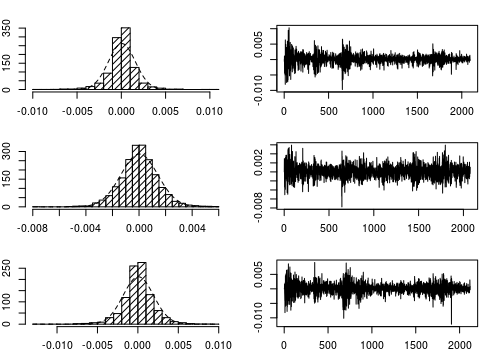
\includegraphics[scale=1]{data2.png}
	\begin{tablenotes}
	\small
	\item Note: The dashed lines in the histograms are probability density functions of the normal distribution with means and standard deviations equal to the means and standard deviations of the corresponding return series.
	\end{tablenotes}
\end{figure}


\subsection{Network models}
The theory of model specification within neural networks is thin, even more so regarding recurrent nets and LSTM's for that matter. Most studies are empirically deciding upon the number of nodes and layers of the networks. Because there are no clear guide lines it has been decided to test two different LSTM models in this thesis. One simple model and one deep model.

\subsubsection{Single layer LSTM model}
The simple LSTM model consists of one hidden layer with 4 LSTM blocks. In the first part of the method, regression forecasting, a linear activation function is used for the output layer \footnote{$g(a) = a$}, in the second part the \textit{sign} function, and in the third part a classification activation function is used, \textit{softmax},

\begin{equation}
\sigma (z)_j = \frac{e^{z_j}}{\sum_{k=1}^K e^{z_k}} \ \ \ \text{for} \ \ j = 1,...,K
\end{equation}

\subsubsection{Deep LSTM model}
The deep LSTM model consists of 3 hidden LSTM layers. The first layer has 4 blocks, the second 50, and the third 100 LSTM blocks. Both the second and the third layer is regularized by a dropout layer which randomly shoots out $50\%$ of all blocks in each step of the epochs. As in the case of the simple LSTM model a linear activation function is again used for the output layer in the first part of the experiment, the sign function in the second part and a softmax function, equation (23), is used in the third part.

\subsection{Time series model}
In this section a time series model is introduced, which can be used in comparison with the neural networks models. This is of course important since the conventional way of analyzing financial time series data is not with neural networks, but rather with time series models.
\\

So, which comparison model is suitable? Arguably one which is rather general but takes the stylized facts about the financial return data into account. It has been decided that because the neural network model operates on lagged inputs of one time step, so will the time series model. In order to catch the autoregressive part of the time series and the non-symmetric conditional movements of the variance an ARMA(1,1)-GJRGARCH(1,1)-process is used. \footnote{The autoregressive moving average model which controls for GARCH variance of order (1,1,1,1) is empirically often used. One example is Gencay \& Stengos (1998) where they compare the model to a simple feedforward neural network.}

\subsection{Results}
\textit{Figure 3} shows the out of sample predictions of the time series model for each index respectively. By visually investigating the predictions there seems to be higher variance in the predictions of the OMX index compared to the other two series. Although the structure of the predictions are similar, where the model is operating around the mean.
\\

\begin{figure}[h]%[H]
\caption{Forecasts with ARMA-GJRGARCH (S\&P 500, Bovespa, OMX). Black indicates the predictions and grey indicates the true returns.}
\centering
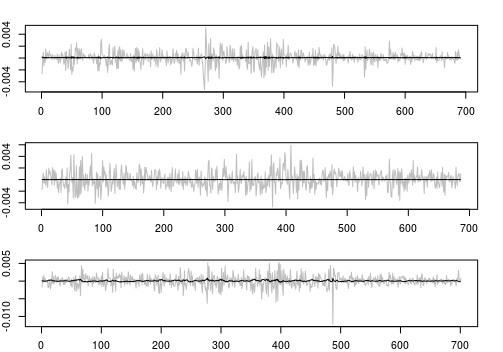
\includegraphics[scale=1]{garch_pred2.png}
\end{figure}

\textit{Figure 4} looks very similar to \textit{figure 3}, but there are some interesting differences. When predicting S\&P 500 the LSTM model seems to have captured the two volatility clusters in the middle of the series better. Although, one cannot say that better capturing the variance necessarily leads to better forecast of the series. Also, the variance of the OMX prediction seems to be uniform with the other predictions, hence not much more volatile as in \textit{figure 3}.
\\

\begin{figure}[h]%[H]
\caption{Predictions from LSTM (S\&P 500, Bovespa, OMX).}
\centering
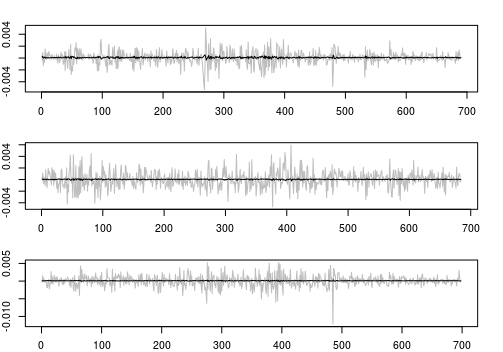
\includegraphics[scale=1]{lstm_pred2.png}
\end{figure}

\textit{Figure 5} is more similar to \textit{figure 4} than \textit{figure 3}. It captures the volatility clusters of the S\&P series as the simple LSTM model. However, the predictions seems to be extremely close the mean.
\\

\begin{figure}[h]%[H]
\caption{Predictions from deep lstm (S\&P 500, Bovespa, OMX).}
\centering
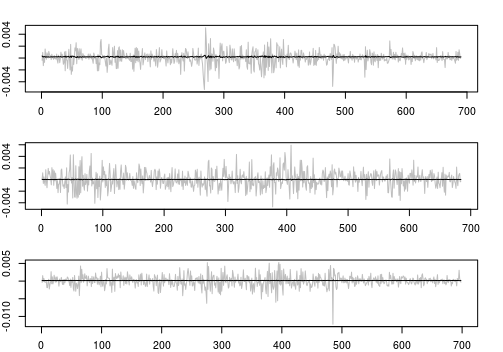
\includegraphics[scale=1]{lstm_deep_pred2.png}
\end{figure}

Furthermore, \textit{figure 6} and 7 are representing the two dimensional output of the softmax activation function yielded by the LSTM and the deep LSTM model. The black lines are representing the estimated probability for a positive return and the grey lines are estimated representing the probabilities for a negative return.\footnote{The black and grey line add up to 1.}
\\

Looking at the figures (6 and 7) one can see that both the LSTM and deep LSTM classifiers always predict positive returns for the S\&P 500 series. This is also true for the deep LSTM model regarding the Bovespa index. Both models are showing a highly non-linear pattern regarding the predictions of the OMX index.

\begin{figure}[h]%[H]
\caption{LSTM forecast output. Black indicates $\mathbf{P}(R>0)$. Grey indicates $1 - \mathbf{P}(R>0)$.}
\centering
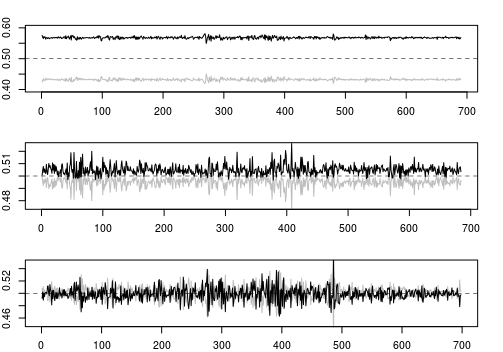
\includegraphics[scale=1]{lstm_prob2.png}
	\begin{tablenotes}
	\item Note: The dashed lines lie at $\mathbf{P}(R>0) = 1 - \mathbf{P}(R>0)$.
	\end{tablenotes}
\end{figure}

\begin{figure}[h]%[H]
\caption{Deep LSTM forecast output. Black indicates $\mathbf{P}(R>0)$. Grey indicates $1 - \mathbf{P}(R>0)$.}
\centering
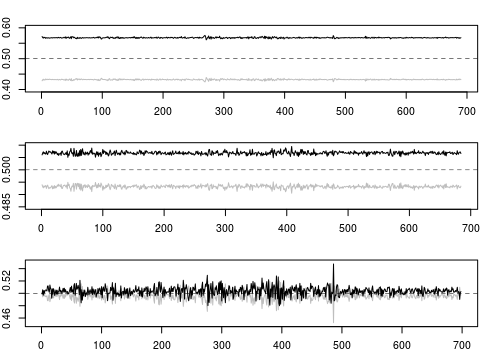
\includegraphics[scale=1]{lstm_deep_prob2.png}
\end{figure}

\subsection{Forecast evaluation}
The regression predictions of the three models looks quite similar. All models have heavily generalized the parameters in order to perform good out of sample predictions and not over-fit to the training dataset. Table 3 shows the sum of squared residuals for each model and each dataset.\footnote{Plots of the residuals are found in the appendix.} The sum of squared residuals are very similar for the models, although the time series model have the lowest sum of squared residuals for the S\&P 500 index.

\begin{table}[h]%[H]
\centering
\caption{Sum of squared residuals from regressions.}
\csvautotabular[separator=semicolon]{sumofsquared.csv}
\end{table}

Recall figures 3, 4 and 5, where the forecasts of the indices are shown. The magnitude is clearly not correct when compared to the true returns. All predictions are very close to the mean value of the series. Hence, in a financial perspective the predictions would be of little use. However, if the predictions are changed slightly and only the direction of the predictions is taken into account, can they be of use from a financial perspective? Yes, if they are able to correctly predict the market directions.
\\

Table 4 shows the percentage of correct directional predictions of all models. This includes the time series model, LSTM model and the deep LSTM model where a sign function is wrapped around the regression output. It also includes the softmax LSTM and the softmax deep LSTM which produce classification output. The bold numbers are the highest correct percentage for each dataset and significant scores of the binomial test are shown with (*) and (**).
\\

\begin{table}[h]%[H]
\centering
\caption{Directional prediction (percentage correct).}
\csvautotabular[separator=semicolon]{TableOfCorrect.csv}
	\begin{tablenotes}
	\small
	\item  (*) significant binomial test at $\alpha=0.90$.
	\item (**) significant binomial test at $\alpha=0.95$.
	\item $H_0$: $p = 50\%$.
	\end{tablenotes}
\end{table}

First note that all models on all datasets are predicting the correct direction with a probability of 50\% or higher. However only four predictions are significant on the out of sample data. For the S\&P 500 index no model yields a significant result. Regarding the Bovespa index only the regular time series model yields a significant results. The interesting observation is when looking at the OMX index. All models predict 52\% correct or better, and the softmax deep lstm predicts over 55\% correct. Note also that the deep LSTM, softmax LSTM and the softmax deep LSTM shows significant forecasts on the direction of the OMX index.

\subsection{Trading strategy evaluation}
The two trading strategies discussed in section 4.1 will be evaluated using the classification prediction, on the out of sample data, from the softmax deep LSTM model and the ARMA-GJRGARCH model. For each index three portfolios will be presented. The first which is the index, i.e. if one buys the index and holds it. The second portfolio will represent the first trading strategy which consists of buying the index when the model predict positive outcomes and staying out of the market when negative returns are predicted. The third portfolio represent the second trading strategy, in which one buys the index when the models predict positive returns and shorts the index when the models predict negative returns. Each portfolio will be based on the starting value of $1$ unit of a given currency.
\\

\begin{figure}[h]%[H]
\caption{Softmax deep LSTM trading strategy.}
\centering
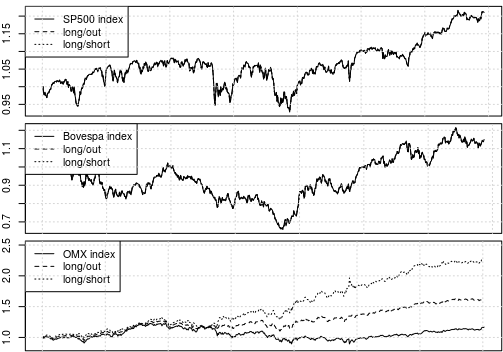
\includegraphics[scale=1]{strategy.png}
\end{figure}

\textit{Figure 8} shows, for each index, the outcomes of the trading strategies based on the softmax deep LSTM model. Recall \textit{figure 7}, where the probability output of the model is shown. Here one can see that the predictions of positive returns for the S\&P 500 index and the Bovespa index are always greater than 0.50. This indicates that the two trading strategies will be identical to these indices. The reason for this is that both strategies buys the index then the model predict positive returns, and if the model always predict positive returns then the strategy always buys index. However, looking at the OMX predictions of \textit{figure 7}, one can see higher dynamics. This clearly shows when the trading strategies are evaluated on the OMX data. Here the first strategy performs around 50\% better than index and the second strategy performs over 100\% better than index. Remember that the out-of-sample data is $33\%$ of the dataset, e.g. the testing data for the OMX index consists of $700$ daily observations.
\\

\textit{Figure 9} has the exact same structure as \textit{figure 8}, the difference is that the ARMA-GJRGARCH model is used in the strategies. The results are unfortunately not as good as the network model. For the S\&P 500 index both strategies perform worse than the index using the time series model. For the Brazilian Bovespa index the second strategy performs worse at the end of the period, although it did perform very well during the first part. The first strategy did outperform the index in the first part but, ended up with the same result in the end. Regarding the OMX index the strategies did worse than the index in the beginning but outperform the index when looking at the total period.

\begin{figure}[h]%[H]
\caption{ARMA-GJRGARCH trading strategy.}
\centering
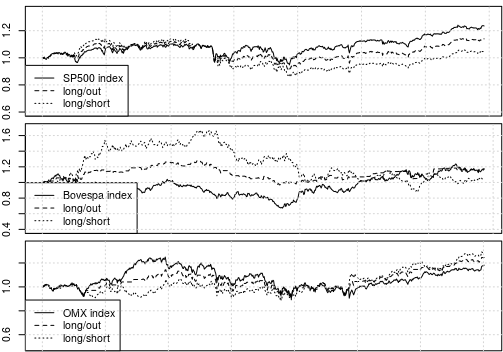
\includegraphics[scale=1]{strategyGARCH.png}
\end{figure}

\newpage

\section{Discussion}
\begin{itemize}
\item Can the American, Brazilian or Swedish stock market returns be predicted using LSTM's?
\end{itemize}
\vspace{0.5cm}

With regards to the magnitude of the regression forecasts of the indices there seems not to be a good way one can predict the stock market returns of the markets with LSTM neural nets.
\\

\begin{itemize}
\item Can the directions of the stock market returns be predicted using LSTM's?
\item Is predictability of market returns different between America, Brazil and Sweden?
\end{itemize}
\vspace{0.5cm}

The network models were not able to predict the direction of the S\&P 500 or Bovespa index with significant result, but three out of four network models did significant predictions on the Swedish OMX index. There is no way of understanding exactly why a neural network model acts the way it does since the parameter space is simply too large. What one can understand is that the network model trains on a dataset, tries to generalize the training, and then predict on an out of sample set. One thought would be that the OMX data has the most similarities between the training and test data. Nevertheless, the results show that the direction of the Swedish market seems to be predictable, whereas the direction of the American and the Brazilian seems not to.
\\

\begin{itemize}
\item Can LSTM neural nets compete with conventional time series models?
\end{itemize}
\vspace{0.5cm}

The simple answer is yes. All the results show that the sequential modeling of a LSTM net is sufficiently sophisticated to yield equal or better result than the famous ARMA-GJRGARCH. Machine learning algorithms for financial and econometric analysis are on the rise, and has been for a long time. These results validates the continuation of that.
\\

\begin{itemize}
\item Is it possible to build a successful financial trading strategy based on LSTM network prediction?
\end{itemize}
\vspace{0.5cm}

A trading strategy based on the regression forecasts would not be advisable. However, a trading strategy based on the directional analysis of a softmax LSTM network might be advisable. As seen in figure 8 the outcomes of the trading strategies are atleast as good as each index. Especially good is the performance on the Swedish market, where the strategies outperforms the market with around 50\% and 100\% respectively. This is of course a spectacular result, which was achieved by consistently better than average prediction and compounding effects over 700 days. As mentioned, the only thing one can be completely sure of is that the model, regarding the OMX index, was able to generalize a pattern that was applicable on the out of sample data. This does not mean that the strategy will work in the future. However, there might be a structure to the smaller Swedish market allowing the model to make these predictions and this needs to be further investigated.
\\

Regarding building a real world trading strategy much more testing would of course be needed. An empirical model specification test would be necessary, where a lot more than two models is tested. In order to improve the model one would want to evaluate and potentially add other input variables, other than exclusively historical returns. Other input variables could be economic indicators such as inflation or other financial data such as exchange rates or other stock market data.

\section{Concluding remarks}
In this thesis it has been shown how LSTM neural networks can be used in order to predict financial returns series, both with a regression approach and a classification approach. It seems to be possible to predict the directions of the Swedish stock market, while it seems not to be possible to predict the US and Brazilian stock market directions. This suggests that the weak form of the efficient market hypothesis does not hold for the Swedish market, while it holds for the US and the Brazilian markets.
\\

These findings may suggest that the American and the Brazilian markets are more data driven compared to the Swedish market. Thus utilize historical data to a higher degree within financial analysis.
\\

The EMH can only be empirically tested, which means that the testing is dependent upon the empirical methodology. LSTM neural network modeling is not a common way of analyzing financial returns. It could well be that the Swedish market has not yet been influenced by neural network modeling to the same degree as the markets which seems to be efficient.
\\

Another suggestion that may explain the fact that the Swedish market seems predictable is purely numerical. It is possible that there are local or global minimums that further reduce the error function of the LSTM networks for the American and the Brazilian markets, although not found with the standard optimization algorithms. This would create the illusion of efficiency of these markets.

\newpage

\section{References}
Bishop M. C. (1995). Neural Networks for Pattern Recognition. Cambridge, UK: Oxford University Press.
\\

Campbell Y. J., Lo W. A., MacKinlay C. A. (1997). The Econometrics of Financial Markets. Princeton, New Jersey: Princeton University Press.
\\

Christoffersen F. P., Diebold X. F., Mariano S. R., Tay S. A., Tse Y. K. (2006). Direction-of-Change Forecasts Based on Conditional Variance, Skewness and Kurtosis Dynamics: International Evidence. Journal of Financial Forecasting 2:1-22.
\\

Cont R. (2000). Empirical properties of asset returns: stylized facts and statistical issues. Quantitative Finance 1:223-236.
\\

Cybenko G. (1989). Approximation by Superpositions of a Sigmoidal Function. Math. Control Signals Systems 2:303-314.
\\

Enders W. (2015). Applied Econometric Time Series. Danvers, MA: John Wiley \& Sons. $4^{th}$ edition.
\\

Enke D. (2005). The Use of Data Mining and Neural Networks for Forecasting Stock Market Returns. Expert Systems with Applications 29:927-940.
\\

Fadlalla A., Lin C. (2001). An Analysis of the Applications of Neural Networks in Finance. Interfaces 31:112-122.
\\

Fama F. E. (1970). Efficient Capital Markets: A Review of Theory and Empirical Work. The Journal of Finance 25:383-417.
\\

Fehrer R., Feuerriegel S. (2015). Improving Decision Analytics with Deep Learning: The
Case of Financial Disclosures. Working paper arXiv:1508.01993.
\\

Gencay R. (1996). Non-linear Prediction for Security Returns with Moving Average Rules. Journal of Forecasting 15:165-174.
\\

Gencay R., Stengos T. (1998). Moving Average Rules, Volume and the Predictability of Security Returns with Feedforward Networks. Journal of Forecasting 17:401-414.
\\

Glosten L. R., Jagannathan R., Runkle D. E.(1993). On The Relation between The Expected Value and The Volatility of Nominal Excess Return on stocks. The Journal of Finance 48:1779-1801.
\\

Griewank A. (2010). Who Invented the Reverse Mode of Differentiation? Documenta Mathematica Extra Volume:389-400.
\\

Hansson, G (1993) Quantitative Structure-Retention Relationships of Diastereomers in Reversed-Phase Liquid Chromatography. Department of Analytical and Marine Chemistry, University of Göteborg and Chalmers University of Technology.
\\

Haykin S. (1998). Neural Networks: A Comprehensive Foundation. Hamilton, Ontario, Canada: Pearson Education. $2^{nd}$ edition.
\\

Hornik K. (1991). Approximation Capabilities of Multilayer Feedforward Networks. Neural Networks 4:251-257.
\\

Hu Y. M., Tsoukalas C. (1999). Combining conditional volatility forecasts using neural networks: an application to the EMS exchange rates. Journal of International Financial Markets, Institutions and Money 9:407-422.
\\

Johnson D. J., Whinston B. A. (1994). Advances in Artificial Intelligence in Economics, Finance and Management. Greenwich, CT:JAI Press.
\\

Maknickiene N., Rutkauskas A. V., Maknickas A. (2011). Investigating of financial market prediction by recurrent neural network. Innovative Infotechnologies for Science, Business and Education 2:3-8.
\\

Mantri K. J., Gahan P., Nayak B. B. (2010). Artifical Neural Networks - An Application to Stockmarket Volatility. International Journal of Engineering Science and Technology 2:1451-1460.
\\

McCulloch S. W.,Pitts W. (1943). A Logical Calculus of the Ideas Immanent in Nervous Activity. Bulletin of Mathematical Biophysics 5:115-133.
\\

Qiu M., Song Y., Akagi F. (2016). Application of Artificial Neural Network for the Prediction of Stock Market Returns: The Case of the Japanese Stock Market. Chaos, Solitons and Fractals 85:1-7.
\\

Roberts H. (1967). Statistical versus Clinical Prediction of the Stock Market. The Center for Research in Security Prices, Chicago: University of Chicago. Unpublished manuscript.
\\

Rosenblatt F. (1962). Principles of Neurodynamics: Perceptrons and the Theory of Brain Mechanisms. Washington, D.C.: Spartan Books.
\\

Rutkauskas A. V., Maknickiene N., Maknickas A. (2010). Modelling of the History and Predictions of Financial Market Time Series Using Evolino. In The $6^{th}$ International Conference “Business and Management 2010”: Selected papers, Vol. 1. Ed. by R. Ginevičius, A. V. Rutkauskas, R. Počs, May 13–14, 2010, Vilnius, Lithuania. Vilnius: Technika, 170–175. doi:10.3846/bm.2010.024
\\

Sewell M. (2011). History of the Efficient Market Hypothesis. UCL Department of Computer Science, Research Note RN/11/04.
\\

Sonoda S., Murata N. (2015). Neural Network with Unbounded Activation Function is Universal Approximator. Faculty of Science and Engineering, Waseda University. Working paper arXiv:1505.03654.



\newpage

\section{Appendix}

\subsection{Numerical packages}
In this thesis Tensorflow, Keras, Rugarch and NetworkX have been used. A short description of the libraries follows in the subsequent subsections.

\subsubsection{Tensorflow \& Keras}
Tensorflow is a library for tensor, i.e. multidimensional arrays, manipulation which has a lot of machine learning functions build in, e.g. neural network training. It was initially released by Google Brain Team in 2015.\footnote{\url{https://www.tensorflow.org/}}
\\

Keras is a high level API running on top of either Deeplearning4j, Tensorflow or Theano.\footnote{\url{https://keras.io/}}

\subsubsection{Rugarch package}
There are several R-packages that can handle time series and GARCH modeling. A few examples are: Rugarch, fGarch, tseries, bayesGARCH, betategarch, dynamo, and rgarch. In this thesis the Rugarch package is used, mostly due to previous experience and recommendations. The Rugarch package is well known in the R-community. It is said to have to most sophisticated optimization, due to its \textit{hybrid} method.
\\

A full description of the Rugarch package can be found at the r-projects website.\footnote{\url{https://cran.r-project.org/web/packages/rugarch/index.html}}
\\

The author of the Rugarch package, Alexios Ghalanos, has also a blog.\footnote{\url{http://unstarched.net/}}

\subsubsection{NetworkX}
Python package NetworkX was used to create the network model (\textit{figure 1}).\footnote{\url{https://networkx.github.io/}}

\subsection{Regression residuals}
Figures 10-12 shows the residuals from the regression modeling of the time series model, the LSTM model and the deep LSTM model.


\begin{figure}
\caption{Residuals from ARMA-GJRGARCH (S\&P 500, Bovespa, OMX).}
\centering
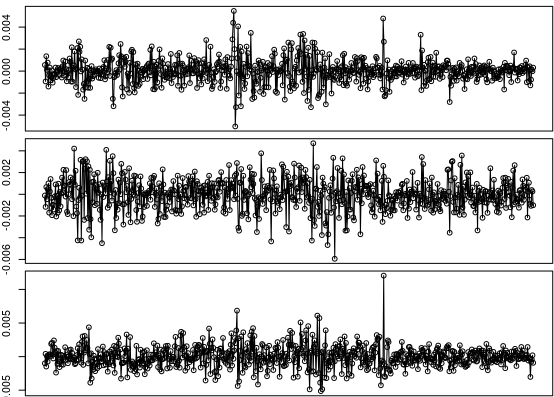
\includegraphics[scale=0.8]{garch_resid.png}
\end{figure}

\begin{figure}[H]
\caption{Residuals from LSTM (S\&P 500, Bovespa, OMX).}
\centering
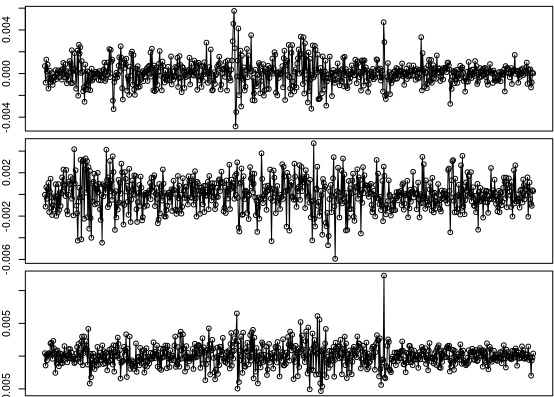
\includegraphics[scale=0.8]{lstm_resid.png}
\end{figure}

\begin{figure}[H]
\caption{Residuals from deep LSTM (S\&P 500, Bovespa, OMX).}
\centering
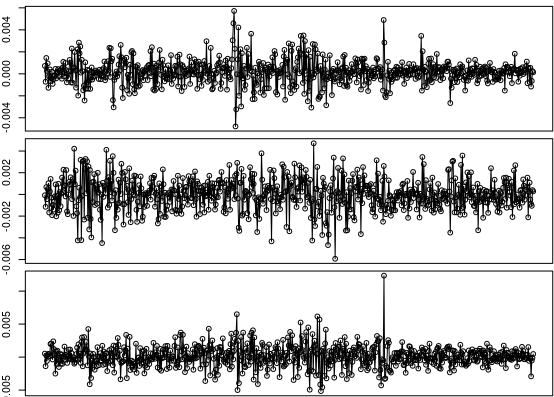
\includegraphics[scale=0.8]{lstm_deep_resid.png}
\end{figure}

%\end{spacing}
\end{document}
